\documentclass[11pt]{article}
\usepackage[letterpaper,top=2cm,bottom=2cm,left=2cm,right=2cm,marginparwidth=1.75cm]{geometry}

 % Useful packages 
\usepackage{hyperref}
\usepackage{biblatex}
\addbibresource{Bib.bib}
\usepackage{mathtools}
\DeclarePairedDelimiterXPP\BigOSI[2]%
  {\mathcal{O}}{(}{)}{}%
  {\SI{#1}{#2}}

\usepackage{amsmath}
\usepackage{empheq}
\usepackage[most]{tcolorbox}
\usepackage{amsmath}
\usepackage{mathrsfs}
\usepackage[utf8]{inputenc}
\usepackage{graphicx}
\usepackage{float}
\usepackage{parskip}
\usepackage{comment}
\usepackage{mhchem}
 \usepackage{tabularx}
 \usepackage{titling}
  \usepackage[explicit]{titlesec}
\usepackage{fancyhdr}
\setlength{\droptitle}{3em} 

\title{Stellar Structure}
\author{Thomas Brosnan}
\date{Notes taken in Professor Kate Maguire's class, Michaelmas Term 2023}

    
\numberwithin{equation}{section}

\newtcbox{\mymath}[1][]{%
    nobeforeafter, math upper, tcbox raise base,
    enhanced, colframe=blue!30!black,
    colback=blue!30, boxrule=1pt,
    #1}

  \newenvironment{bux}
    {
    \empheq[box=\tcbhighmath]{align}
   }{
    \endempheq
    }
    \newenvironment{bux*}
    {
    \empheq[box=\tcbhighmath]{align*}
   }{
    \endempheq
    }
\newcommand{\hsp}{\hspace{8pt}}

\newcommand*{\sectionFont}{%
  \LARGE\bfseries
}

\makeatletter
\let\Title\@title % Copy the title to a new command
\makeatother

%change this RGB value to change the section background colour 
\definecolor{mycolor1}{RGB}{74, 241, 130}
\colorlet{SectionColour}{mycolor1}
%subsection background colour 
\definecolor{mycolor2}{gray}{0.8}
\colorlet{subSectionColour}{mycolor2}
%subsubsection background colour 
\definecolor{mycolor3}{RGB}{255,255,255}
\colorlet{subsubSectionColour}{mycolor3}




    
\begin{document}

\maketitle

\newpage
\tableofcontents
% For \section
 \titleformat{\section}[block]{\sectionFont}{}{0pt}{%
 \fcolorbox{black}{SectionColour}{\noindent\begin{minipage}{\dimexpr\textwidth-2\fboxsep-2\fboxrule\relax}\thesection  \hsp #1 {\strut} \end{minipage}}}
% For \subsection
 \titleformat{\subsection}[block]{\bfseries}{}{0pt}{%
 \fcolorbox{black}{subSectionColour}{\noindent\begin{minipage}{\dimexpr\textwidth-2\fboxsep-2\fboxrule\relax}\thesubsection  \hsp #1 {\strut} \end{minipage}}}
% For \section*
 \titleformat{name=\section, numberless}[block]{\sectionFont}{}{0pt}{%
 \fcolorbox{black}{SectionColour}{\noindent\begin{minipage}{\dimexpr\textwidth-2\fboxsep-2\fboxrule\relax} #1 {\strut} \end{minipage}}}
  % For \subsection*
 \titleformat{name=\subsection, numberless}[block]{\bfseries}{}{0pt}{%
 \fcolorbox{black}{subSectionColour}{\noindent\begin{minipage}{\dimexpr\textwidth-2\fboxsep-2\fboxrule\relax} #1 {\strut} \end{minipage}}}
 % For \subsubsection
 \titleformat{\subsubsection}[block]{\bfseries}{}{0pt}{%
 \fcolorbox{black}{subsubSectionColour}{\noindent\begin{minipage}{15cm}\thesubsubsection \hsp #1 {\strut} \end{minipage}}}
  % For \subsubsection*
 \titleformat{name=\subsubsection, numberless}[block]{\bfseries}{}{0pt}{%
 \fcolorbox{black}{subsubSectionColour}{\noindent\begin{minipage}{15cm} #1 {\strut} \end{minipage}}}
\newpage
%header 
\pagestyle{fancy}
\fancyhf{} % Clear all header and footer fields
\fancyhead[L]{\Title}
\fancyhead[R]{\nouppercase{\leftmark}}
\fancyfoot[C]{-~\thepage~-}
\renewcommand{\headrulewidth}{1pt}





\normalsize
\newpage
\tcbset{highlight math style={boxsep=5mm,colback=red!0!blue!0!green!0!}}

\section{Observable properties of stars}

\subsection{Luminosity}
\begin{itemize}
    \item Is the total energy emitted per unit time (power). To calculate this we add up all the flux (energy passing through unit area $dA$ per unit time $dt$) over all the different wavelengths. This makes it become an integral:
\begin{empheq}[box=\tcbhighmath]{equation}
\begin{split}
   L = 4 \pi R^2\int_0^{\infty} F_{\lambda}d\lambda
\end{split}
\end{empheq}

\end{itemize}
\subsection{Parallax}
\begin{itemize}
    \item Is the apparent motion of an object with respect to the background due to the motion of the observer. This can allow us to calculate the distance to stars, as the motion of the earth around the sun is well measured. This results in the notion of a parsec which is the distance to a star that creates a parallax angle of 1 arc-second:
\begin{empheq}[box=\tcbhighmath]{equation} 
\begin{split}
   p (arcsecond) = \frac{1 Au}{d (parsec)}
\end{split}
\end{empheq}
\end{itemize}
\subsection{Magnitudes} 
\begin{itemize}
    \item  The apparent magnitude is a measure of brightness of a star as seen from earth, based on some reference in the same filter: 
\begin{empheq}[box=\tcbhighmath]{equation}
\begin{split}
  m = -2.5 \log_{10}(\frac{F}{F_0})
\end{split}
\end{empheq}
\item Absolute magnitude is the magnitude an object would have at a distance of 10 pc from the object: 
\begin{empheq}[box=\tcbhighmath]{equation}
\begin{split}
   M -m = -5\log_{10}(\frac{d}{10})
\end{split}
\end{empheq}
\end{itemize}

\subsection{Effective temperature}
\begin{itemize}
    \item Stars are assumed to be emitting as black bodies in thermodynamic equilibrium. Thus their spectral radiance is given by the Plank function:
\begin{empheq}[box=\tcbhighmath]{equation}
\begin{split}
   B_{\lambda}(T) = \frac{2hc^2}{\lambda^5}\frac{1}{e^{\frac{hc}{\lambda k_b T}}-1}
\end{split}
\end{empheq}
\item This can be differentiated to get Wien's law:
\begin{empheq}[box=\tcbhighmath]{equation}
\begin{split}
  \lambda_{peak} T = 0.0029 ~Km
\end{split}
\end{empheq}
\item One can also integrate this equation over all wavelengths to obtain the Stefan Boltzmann law:
\begin{empheq}[box=\tcbhighmath]{equation}
\begin{split}
   F_{tot} = \sigma T^4
\end{split}
\end{empheq}
Where sigma is the Stefan Boltzmann constant. 
\item This means that the bolometric luminosity is:
\begin{empheq}[box=\tcbhighmath]{equation}
\begin{split}
  L =4 \pi R^2 \sigma T^4
\end{split}
\end{empheq}

\end{itemize}

\subsection{Stellar types}
\begin{itemize}
    \item See Galactic structure notes.
\end{itemize}

\subsection{Colour temperature}
\begin{itemize}
    \item Another way of classifying stars based on temperature. Colour is chosen based on the filter in which there black body peak is. 
\end{itemize}

\subsection{Excitation temperature}
\begin{itemize}
\item The excitation energy is the minimum amount of energy required to promote a specific electron from its ground state to a higher energy level within an atom or molecule. 

Then the relative number of atoms with electrons in different states is given by the Boltzmann equation:
\begin{empheq}[box=\tcbhighmath]{equation}
\begin{split}
  \frac{N_b}{N_a} = \frac{g_b}{g_a}\frac{e^{-\frac{E_b}{k_bT}}}{e^{-\frac{E_a}{k_aT}}} = \frac{g_b}{g_a}e^{-\frac{(E_b-E_a)}{k_bT}}
\end{split}
\end{empheq}
Here $g_n = 2n^2$ and $E_n = -\frac{13.6Ev}{n^2}$. 



\end{itemize}
\subsection{Ionisation energy}
\begin{itemize}
    \item Is related to the energy needed to produce a given ratio between the populations of two ionisation stages. 

This ratio is defined by the Saha equation:
\begin{empheq}[box=\tcbhighmath]{equation}
\begin{split}
  \frac{N_{i+1}}{N_i} = \frac{2Z_{i+1}}{n_eZ_i}(\frac{2\pi m_e k_bT}{h^2})e^{-\frac{\chi}{k_bT}}
\end{split}
\end{empheq}
Here $Z_i=\sum_{j=1}^{\infty}g_je^{-\frac{(E_j-E_1)}{k_bT}}$, sums over all possible ways an atom can be stripped of an electron. 

\end{itemize}
\subsection{Optical opacity}
\begin{itemize}
    \item See Galactic structure notes
\end{itemize}

\subsection{Photosphere} 
\begin{itemize}
    \item This is the optically thick boundary of an astrophysical body and is defined as the region from which the photons were last scattered. (i.e. where the light appears to come from). Mathematically this is the depth into the star at which the optical depth is $\tau_{\lambda}=2/3$, averaged over the star.  Notably this is not the top of the atmosphere.  
\end{itemize}

\subsection{Absorption types}
\subsubsection{Bound-bound}
\begin{itemize}
    \item This is when a photon is absorbed by an atom, resulting in an electron becoming excited but not ionised. No simple equation for describing contribution to opacity. 
\end{itemize}
\subsubsection{Bound-free} 
\begin{itemize}
    \item This is when a photon is absorbed by an atom resulting in an electron becoming ionised, equation is relatively simple to write down for $H$ but becomes harder after that. 
\end{itemize}
\subsubsection{Free-free}
\begin{itemize}
    \item This is when a free electron absorbs a photon in passing an ion. As it passes the ion it is accelerated, absorbing a photon in the process. 
\end{itemize}

\subsubsection{Electron scattering }
\begin{itemize}
    \item This is an elastic collision between two particles i.e. photon and an electron. If $hf << m_ec^2$ then the electron will be relatively unmoved by the collision resulting in only the direction of the photon being altered. This is the dominant source of opacity in stellar interiors.  
\end{itemize}
\begin{itemize}
    \item The total opacity is the sum of all these contributions.  For treating the interior of stars we can combine all these sources and integrate over all wavelengths, to give the mean opacity that depends only on composition, density and temperature.  The results of this are usually approximated as:
\begin{empheq}[box=\tcbhighmath]{equation}
\begin{split}
  \kappa = \kappa_0 \rho^{\alpha}T^{\beta}
\end{split}
\end{empheq}
Where $\alpha$ and $\beta$ are slowly varying functions of density and temperature and $\kappa_0$ is a constant for a given chemical composition.

\end{itemize}

\newpage

\section{Equations of stellar structure}
\subsection{Assumption and variables for stellar structure}
\begin{itemize}
    \item Here we will assume we are dealing with an isolated body with spherical symmetry (thus our only variable is $r$), (local) thermodynamic equilibrium and we will ignore for now, rotation, magnetic fields and time dependence. 

\item The variables we will be considering are Radius $r$, Mass $m(r)$, Luminosity $L(r)$, Pressure $P(r)$, Temperature $T(r)$, Density $\rho(r)$ and Composition $X_i(r)$. 
\end{itemize}

\subsection{Mean free path}
\begin{itemize}
    \item For a particle moving with a speed $v$ over a time $t$, the mean free path is defined as the distance traveled, divided by the number of collisions. So if $\sigma=\pi r^2$ is the cross-sectional area of an atom with radius $r = 2a_0$, as the radius is twice the Bohr radius $a_0$ and $n$ is the number density of the particles, then the mean free path is given by:
\begin{empheq}[box=\tcbhighmath]{equation}
\begin{split}
  \lambda = \frac{vt}{n\sigma vt} = \frac{1}{n\sigma} = \frac{1}{4 \pi n a_0^2}
\end{split}
\end{empheq}
\end{itemize}

\subsection{Hydrostatic equilibrium}
\begin{itemize}
\item In order for a star to not collapse under its own gravity, there must be a certain pressure that negates gravity and keeps material static.  It can be proved that in order for this to hold we must have that for the pressure:
\begin{empheq}[box=\tcbhighmath]{equation}
\begin{split}
 \frac{dP_r}{dr} = -G\frac{M_r\rho_r}{r^2}
\end{split}
\end{empheq}
Where $\rho_r$ is the density enclosed with in a radius $r$. Hydrostatic equilibrium is essentially momentum conservation.
\end{itemize}

\subsection{Mass Continuity}
\begin{itemize}
\item If we consider a infinitesimal thin shell of thickness $dr$ then the volume $dV$ is $dV = 4 \pi r^2 dr$, so the mass is $dM = 4 \pi r^2 \rho_r dr$, so the mass conservation equation is: 
\begin{bux}
    \begin{split}
         \frac{dM_r}{dr} = 4\pi r^2\rho_r
    \end{split}
\end{bux}
This is the second equation of stellar structure 
\end{itemize}


\subsection{Minimum central pressure of a star }
\begin{itemize}
    \item Dividing the first stellar equation by the second 
\begin{bux}
    \begin{split}
        \frac{dP}{dM} = \frac{GM}{4\pi r^4}
    \end{split}
\end{bux}
Then we can integrate from the center to the surface and notice that since $r_{surface}>r$ for all $r$ and $P_{surface} =0$, then:
\begin{bux}
    \begin{split}
        P_{center}-P_{surface} &= \int_{0}^{M_{surface}}\frac{GM}{4\pi r^4}dM > \int_{0}^{M_{surface}}\frac{GM}{4\pi r_{surface}^4}dM  \\
& \implies P_{center} > \frac{GM^2}{8\pi R^4}
    \end{split}
\end{bux}
\end{itemize}

\subsection{Mean molecular weight}
\begin{itemize}
    \item We can think of this quantity as the average mass of the particles present in units of the mass of  a hydrogen atom.  For a neutral gas it is defined as: 
\begin{bux}
    \begin{split}
        \mu_n = \frac{\sum_j N_j \frac{m_j}{m_H}}{\sum_jN_j} = \frac{\bar{m}}{m_H}
    \end{split}
\end{bux}
Here we are summing over all the different types of atoms $j$, with $N_j$ being the number of each of those atoms there are and $m_j$ their mass. 
For an ionised gas the mean molecular mass becomes: 
\begin{bux}
    \begin{split}
        \mu_i = \frac{\sum_j N_j \frac{m_j}{m_H}}{\sum_jN_j(1+z_j)}
    \end{split}
\end{bux}
Where $z_j$ is the number of electrons the atom $j$ looses in the process of ionisation.  Handily we can then write the ideal gas law in terms of this mean molecular weight seeing as the mean mass $\bar{m}$ is related to $\mu$ by $\bar{m}= m_H \mu$, so :
\begin{bux}
    \begin{split}
        P = nkT = \frac{\rho kT}{\bar{m}} = \frac{\rho kT}{\mu m_H}
    \end{split}
\end{bux}

\end{itemize}

\subsection{Central temperature of a star} 
\begin{itemize}
    \item We can now use this expression as well as the minimum central pressure to calculate the minimum central temperature. If we assume the pressure is constant through out the star then $\rho = M/\frac{4}{3}\pi R^3$, then: 
\begin{bux}
    \begin{split}
        T_{center}= \frac{\mu m_H P_{center}}{\rho k} > \frac{\mu m_H GM}{kR}
    \end{split}
\end{bux}
\end{itemize}
\subsection{Radiation pressure}
\begin{itemize}
    \item The total pressure in a star comes from the pressure of the gas and the radiation pressure. The radiation pressure $P_{rad}$ is given by:
\begin{bux}
    \begin{split}
        P_{rad} = \frac{1}{3} a T^4
    \end{split}
\end{bux}
Where $a$ is the radiation constant $a = 7.676 \times 10^{-16}~ Jm^{-3}K^{-4}$. The radiation pressure is only really relevant in high mass stars, only makes up $0.1\%$ of the pressure in the sun. 
\end{itemize}

\subsection{Energy conservation in a star }
\begin{itemize}
    \item The contribution of $dM_r$ to the change in luminosity is $dL_r = \epsilon_rdM_r$, where $\epsilon_r$ is the total energy released per unit mass per unit time. Then using the second equation of stellar structure $ dM_r = 4\pi r^2\rho_rdr$, so:
\begin{bux}
    \begin{split}
         \frac{dL_r}{dr} = 4\pi r^2\rho_r \epsilon_r
    \end{split}
\end{bux}
This is the third equation of stellar structure. 
\end{itemize}

\subsection{Virial theorem}
\begin{itemize}
    \item If we take the first equation of stellar structure and multiply it by $4\pi r^3dr$ and integrate from center to surface, then we get: 
\begin{bux}
    \begin{split}
        \int_c^s4\pi r^3dP_r = - \int_c^s\frac{GM}{r}4\pi r^2\rho_rdr
    \end{split}
\end{bux}
Then we integrate by parts the LHS and notice that the RHS can be simplified with $4 \pi r^2 \rho_rdr = dM_r$, so: 
\begin{bux}
    \begin{split}
        4 \pi[r^3P_r]_c^s -3 \int_c^s4P_r\pi r^2dr = - \int_c^s\frac{GM}{r}dM_r
    \end{split}
\end{bux} 
But since the radius at the center is $0$ and the pressure at the surface is $0$ so the first term vanishes.  Also the RHS can be recognised as the total gravitational energy $\Omega$. For the last integral we consider an ideal monoatomic gas for which the internal energy per unit volume is $u = \frac{3}{2}nkT = \frac{3}{2}P$.  So the RHS becomes: 
\begin{bux}
    \begin{split}
        -3 \int_c^s4P_r\pi r^2dr  = -2 \int_0^R4u\pi r^2dr = -2U 
    \end{split}
\end{bux}
Where here $U$ is the total internal energy of the star. Thus the two sides have become:
\begin{bux}
    \begin{split}
\label{eqn:2.15}
        \Omega = -2U
    \end{split}
\end{bux}
And since $E = \Omega + U$, then either $E=-U$ or $E = \frac{\Omega}{2}$. This is the Virial theorem.  The implications of this theorem is that if stars are able to convert potential energy $\Omega$ into internal energy $U$ they will then heat up and radiate away a certain amount of this energy.  $E_{rad}$ is then either $-\frac{1}{2}\Delta \Omega$ or $\Delta U$.  So half the energy from contraction is used the heat up the star and half of it is radiated away.  After the star has radiated energy away it cool and contracts repeating the process. 
\end{itemize}

\subsection{Kelvin-Helmholtz timescale}
\begin{itemize}
    \item This is the characteristic time scale on which a star radiates all its thermal energy. For a star of mass $M$ and radius $R$, since $E_{rad} = -\frac{1}{2} \Delta \Omega= \frac{3GM^2}{10R}$, then:
\begin{bux}
    \begin{split}
        t_{kH} = \frac{E_{rad}}{\bar{L}} = \frac{3GM^2}{10R\bar{L}}
    \end{split}
\end{bux}
If we calculate this for our sun we see it is far shorter then how old the sun all ready is so this is clearly not the whole story. 
\end{itemize}

\subsection{Nuclear fusion} 
\begin{itemize}
    \item The total mass of the nucleus of an atom $M(Z,N)$ is always less than the mass of the $Z$ protons and $N$ neutrons that make it up. This means that when we fuse atoms energy is released. This energy is called the binding energy and given by: 
\begin{bux}
    \begin{split}
         Q(Z,N) = \left[ Zm_p + Nm_n - M(Z,N)\right]c^2
    \end{split}
\end{bux}
For 4 hydrogen atoms fusing to helium the fractional energy change is:
\begin{bux}
    \begin{split}
        \frac{\Delta E}{E} = \frac{4m_pc^2-m_{He}c^2}{4m_pc^2} = 0.007
    \end{split}
\end{bux}
\item Two charged particles need to over come the coulomb force to fuse, using, this happens when:
\begin{bux}
    \begin{split}
        E = \frac{3}{2}kT = \frac{1}{4 \pi \epsilon_0}\frac{Z_1Z_2e^2}{r}
    \end{split}
\end{bux}
The temperature need for this is then $T \approx 10^{10}K$ but the central temperature of the sun is roughly $10^7$, so something is clearly wrong. This is where we need quantum tunneling. Due to the uncertainty principle a particle has a finite probability of overcoming a potential barrier, allowing fusion to happen at lower temperatures. 

\item  Due to nuclear fusion we can get the nuclear timescale for a star to radiate away all its energy
\begin{bux}
    \begin{split}
        t_{nuc} = \frac{E_{nuc}}{\bar{L}} = \frac{0.007Mc^2}{\bar{L}}
    \end{split}
\end{bux}
This gives a better answer to how long the sun will live. 

\end{itemize}


\subsection{Radiation transfer in the sun}
\begin{itemize}
    \item The mean free path can be defined as $\lambda = 1/n\sigma = 1/\bar{\kappa}\rho$.  For a random walk the displacement $d$ of a photon is given by:
\begin{bux}
    \begin{split}
        d = \lambda \sqrt{N}
    \end{split}
\end{bux}
Where $N$ is the number of mean free paths travelled.  The time taken to then random walk from the center of the star to the surface is called the diffusion time and is given by:
\begin{bux}
    \begin{split}
        t_{diff} = \frac{N\lambda}{c} = \frac{R^2}{\lambda c}
    \end{split}
\end{bux}
\end{itemize}

\subsection{Energy transport by radiation}
\begin{itemize}
    \item We can take an diffusive approach, In spherical symmetry for particles the particle flux $j$ is given by: 
\begin{bux}
    \begin{split}
        j = -D\frac{dn}{dr}
    \end{split}
\end{bux}
Where $n$ is the number density of particles and $D=\frac{1}{3}v\lambda$ is the diffusion coefficient ($v$ here is velocity). For radiation the flux of radiative energy $F_r$ at radius $r$ is: 
\begin{bux}
    \begin{split}
        F_r = - D\frac{dU_r}{dr}
    \end{split}
\end{bux}
Where $U_r$ is the photon energy density, given by $U = aT^4$, assuming the radiation field inside a star can be described by a black body.  $D$ is once again the diffusion coefficient and is given by $D = \frac{1}{3}c \lambda = \frac{c}{3 \bar{\kappa}\rho_r}$, Thus the full expression is: 
\begin{bux}
    \begin{split}
        F_r = -\frac{4acT^3_r}{3\bar{\kappa}\rho_r}\frac{dT_r}{dr}
    \end{split}
\end{bux}
The using the equation for the radiative flux as a function of luminosity, $F = L/4 \pi r^2$, Then: 
\begin{bux}
    \begin{split}
\label{stellar4}
        \frac{dT_r}{dr} = - \frac{3 \bar{\kappa} \rho_r}{16\pi acr^2T_r^3}L_r
    \end{split}
\end{bux}
This is the 4th equation of stellar structure.  If we instead look at energy transfer via convection we can show that convection will happen if:
\begin{bux}
    \begin{split}
        \left| \frac{dT}{dr}\right| > \left| \left( 1-\frac{1}{\gamma}\right)\frac{T}{P}\frac{dP}{dr}\right|
    \end{split}
\end{bux}
Where $\gamma$ is the adiabatic exponent $\frac{C_P}{C_V}$, the ratio of heat capacities.  Convection takes place on the surface of low mass stars but high mass stars will have core convection. 
\end{itemize}

\subsection{Polytropic solutions}
\begin{itemize}
    \item The standard equation of state is that the pressure in a star is just equation for an ideal Gas plus the radiation pressure. This takes the form: 
\begin{bux}
    \begin{split}
        P  = \frac{\rho k_B T}{\mu m_H} + \frac{1}{3}a T^4
    \end{split}
\end{bux}
\item To make this more accurate we would like to be able to solve the equations of stellar structure for the four variables $P, M, L$ and $T$, however the lack of boundary conditions for $P$ and $T$ at the center of a star make this impossible. 

\item To fix this we replace this equation with a polytrope that is assuming the pressure is equal to some power of $\rho$ indexed by the polytropic index $n$:
\begin{bux}
    \begin{split}
        P = K \rho^{\gamma} = K \rho^{1 + \frac{1}{n}}
    \end{split}
\end{bux}
Where $K$ is a constant and $\gamma$ is the adiabatic index, which by the equipartition theorem is $\gamma = 1 + \frac{2}{f}$, where $f$ is the degrees of freedom of a single molecule. For an ideal gas $f=3$ so $\gamma = 5/3$. This is assuming a non-relativistic gas, for relativistic gas $\gamma = 4/3$. 
\end{itemize}

\subsection{Eddington luminosity}
\begin{itemize}
    \item Assuming that the pressure in a very large star is dominated by radiation pressure with no convection, then the maximum Luminosity a star can have and still remain in hydrostatic equilibrium can be found from the following:
\begin{bux}
    \begin{split}
        P = P_{rad} = 1/3aT^4 ~~ \implies \frac{d P}{dr} = \frac{4}{3}aT^3\frac{dT}{dr}
    \end{split}
\end{bux}
Then using stellar equation \ref{stellar4} and solving for the Luminosity results in:
\begin{bux}
    \begin{split}
        L = \frac{4\pi c G M}{\bar{\kappa}}
    \end{split}
\end{bux}

\end{itemize}

\newpage
\section{Star Formation }
\subsection{Collapse of clouds}
\begin{itemize}
    \item Stars form in dark dusty clouds in interstellar space. Gas between the stars is called the \emph{interstellar medium}. It is easiest for stars to collapse when cold and dense. Molecular clouds (mainly $H_2$) are very cold ($10-30K$ ) and dense $\sim 1 \times 10^8 - 1 \times 10^{10}~~ m^{-3}$.  We can use the Virial theorem for an ideal gas, $2U+\Omega=0 $, the same as discussed earlier for stellar interior\ref{eqn:2.15}. From this we see that if $2U<|\Omega|$ then gravity will win and a cloud of gas will collapse.  

\end{itemize}

\subsubsection{Jeans Mass}
\begin{itemize}
    \item This is the minimum mass a cloud of Gas with constant density $\rho$ Can have and still initiate spontaneous gravitational collapse.  Using the Virial theorem, it can be shown that this mass is: 
\begin{bux}
    \begin{split}
\label{eqn:3.1}
        M_J = \left(\frac{5k_BT}{G\mu m_{H}} \right)^{3/2} \left(\frac{3}{4 \pi \rho} \right) ^{1/2}
    \end{split}
\end{bux}
This can also be turned into the minimum radius that still results in collapse of a cloud, known as the \emph{Jeans length}: 
\begin{bux}
    \begin{split}
        R_J =  \left( \frac{15k_BT}{4 \pi G \mu m_H \rho}\right)^{1/2} 
    \end{split}
\end{bux}
\end{itemize}
\subsubsection{Converted Gravitational energy}
\begin{itemize}
\item Converted Gravitational energy cannot stop this collapse. As collapse happens the internal energy increases but not all of this turns into kinetic energy. There are rotational modes of the molecules as well as excitation of the electrons to different energy levels. Since de-excitation emits photons mainly at IR and mm- wavelengths to which the cloud is transparent to, this energy does not stay in the cloud, allowing further contraction to proceed. 
\end{itemize}

\subsubsection{Fragmentation }
\begin{itemize}
    \item As a cloud collapses the density increases rapidly, by equation \ref{eqn:3.1} the Jeans mass then decreases. This allows portions of the cloud to separate themselves from the rest and collapse on their own. This can form multiple stars. 
\end{itemize}

\subsection{Protostars }
\begin{itemize}
    \item A protostar is a very young star that is taking in mass from its parent star-forming cloud. It contracts and heats until the core temperature is sufficient for hydrogen fusion.  Protostars appear above the main sequence as they are larger then main sequence stars while still collapsing. Luminosity decreases even as its temperature rises because it is becoming more compact. 
\end{itemize}


\subsection{The Main sequence }
\begin{figure}[H]
\centering
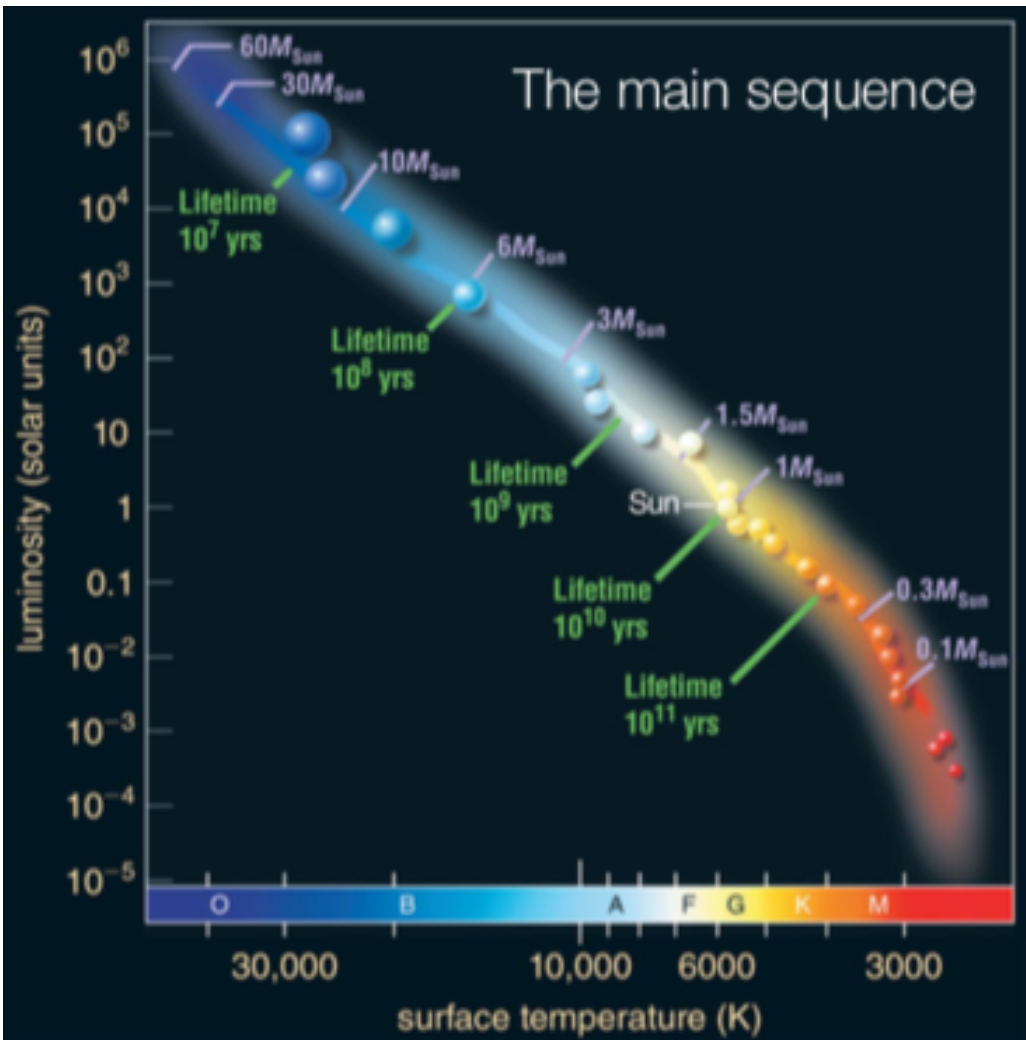
\includegraphics[width=0.6\textwidth]{Graph2.png}
\caption{\label{fig:2}\emph{Main sequence lifetimes }}
\end{figure}
\begin{itemize}
    \item The main sequence is defined as all stars that are fusing Hydrogen in their cores.  Equating the ideal gas law and our central pressure approximations we get that $T \propto \mu M/R$. The Minimum temperature for fusion is $T > 5 \times 10^6 K$ which corresponds to a mass of $\sim 0.08 M_{\odot} $. Below this mass are brown dwarfs which hh-=ave no sustained fusion and are thus not stars. 

\item There is also a measured relationship relation the mass of a star and its radius on the main sequence. This comes from \url{https://www.daviddarling.info/encyclopedia/M/mass-radius_relation.html} and is as follows: 
\begin{bux}
    \begin{split}
        R \propto M^{0.8}
    \end{split}
\end{bux}
\end{itemize}










\begin{figure}[H]
\centering
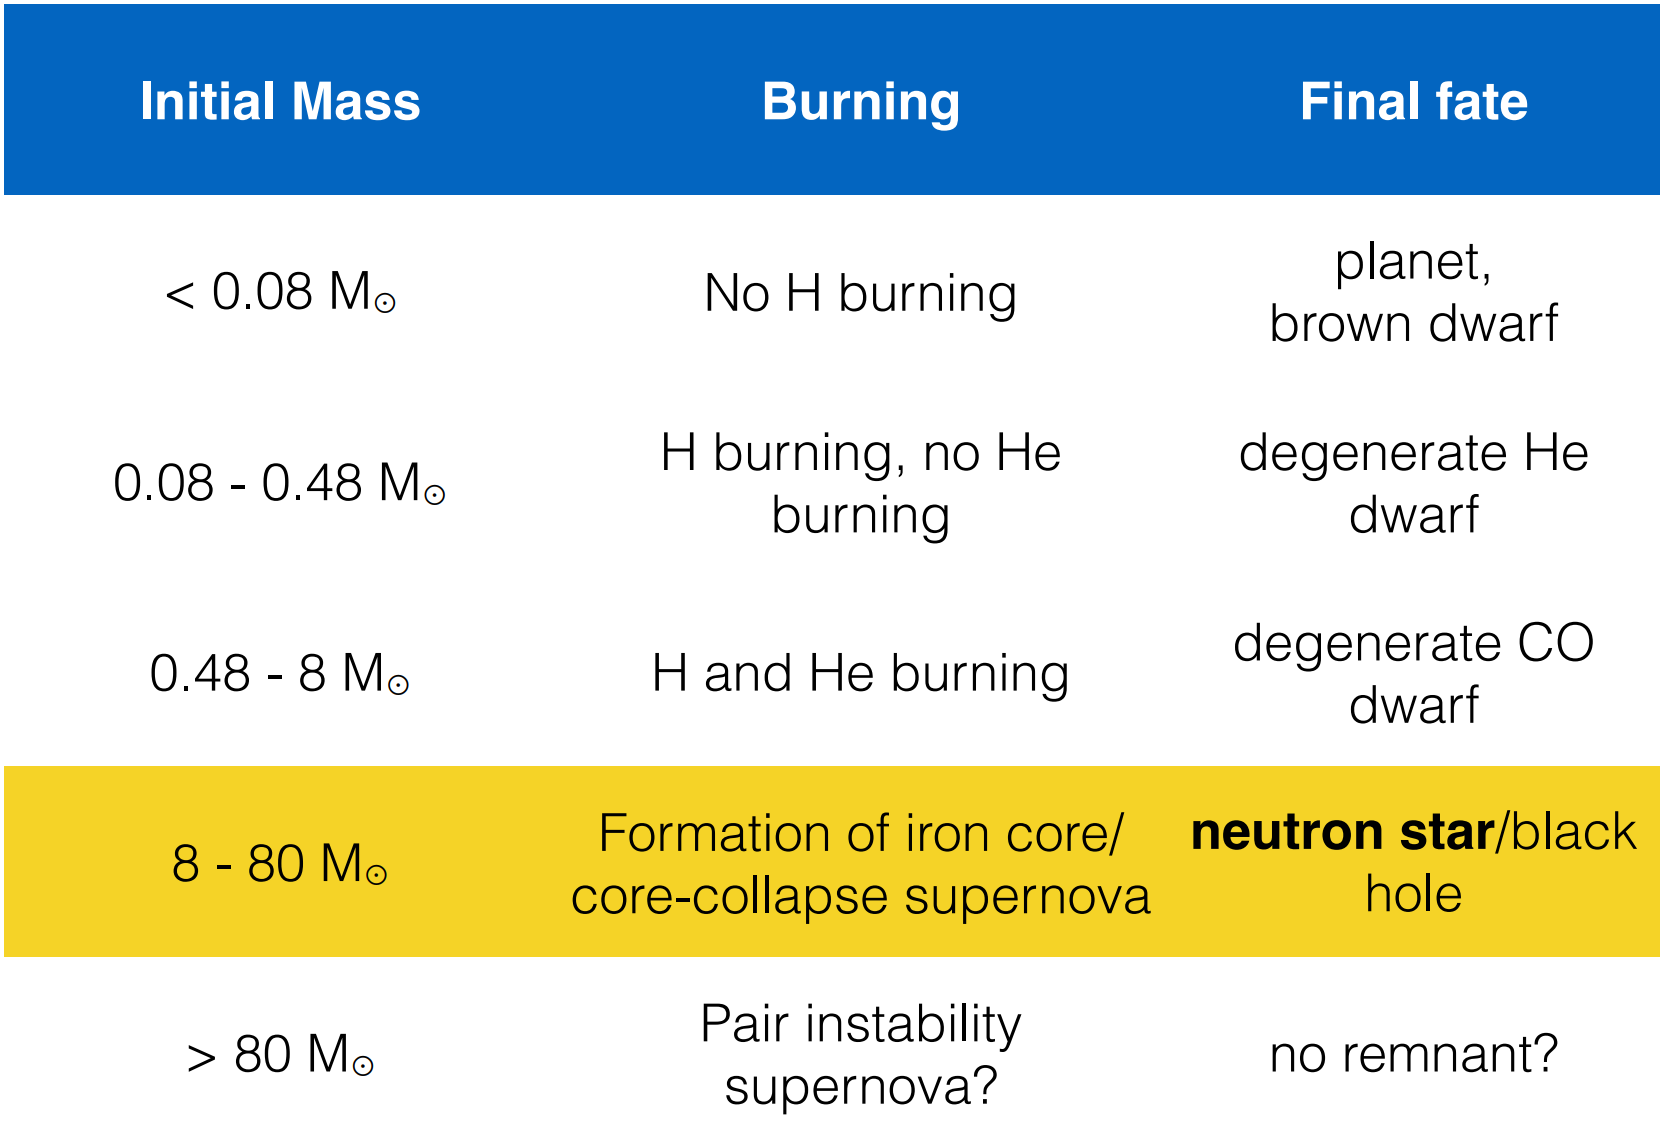
\includegraphics[width=0.6\textwidth]{image.png}
\caption{\label{fig:2}\emph{Flattening out of a galaxies spectrum}}
\end{figure}





\end{document}
